\documentclass{beamer}
\usetheme{Boadilla}
\usecolortheme{spruce}


\usepackage[english]{babel}
\usepackage[utf8x]{inputenc}
\usepackage{amsmath, amssymb, amsthm, textcomp, graphicx, subcaption, siunitx}
\usepackage{algorithm}
\usepackage[noend]{algpseudocode}

\renewcommand{\l}{\left}
\renewcommand{\r}{\right}
\newcommand{\reals}{\mathbb{R}}
\newcommand{\rationals}{\mathbb{Q}}
\newcommand{\naturals}{\mathbb{N}}
\newcommand{\integers}{\mathbb{Z}}
\newcommand{\complex}{\mathbb{C}}

\graphicspath{ {./images/} }

\title{The Three Body Problem}
\author[]{Michael Dymek}
\institute[]{Western Washington University}
\date{June 2nd 2021}

\begin{document}
\begin{frame}
	\titlepage
\end{frame}

\begin{frame}
\frametitle{The Three Body Problem}
Given the initial positions and velocities of three point-masses, determine how the positions of each body evolves over time. \bigskip

This problem does not have a general analytic solution the way that two bodies does.
\end{frame}



\begin{frame}
\frametitle{Theory}
When solving for the motion of an object under given forces, we use Newton's second law
\[ \vec{a} = \frac{\vec{F}}{m}. \]
Between any two bodies, the gravitational force between them is
\begin{equation*}
	F_G = \frac{G m_1 m_2}{r^2}\hat{r},
\end{equation*}
where $G = \SI{6.67e-11}{\newton \meter^2 \per \kilo \gram^2}$ is the gravitational constant.
\end{frame}

\begin{frame}
\frametitle{Theory}
Then, for an arbitrary $n$ number of bodies, we can calculate the $x$ and $y$ components of acceleration using the following formula. The gravitational force acting on the $u^{\text{th}}$ body is
\begin{align*}
	\vec{F}_{x,u} &= \sum_{u \neq v} \frac{G m_v m_u}{r_{u,v}^2} \frac{\Delta x_{u,v}}{r_{u,v}} = \sum_{u \neq v} \frac{G m_v m_u\Delta x_{u,v}}{r_{u,v}^3} \\
	F_{y,u} &= \sum_{u \neq v} \frac{G m_v m_u}{r_{u,v}^2} \frac{\Delta y_{u,v}}{r_{u,v}} = \sum_{u \neq v} \frac{G m_v m_u \Delta y_{u,v}}{r_{u,v}^3}
\end{align*}
This is shown for two dimensions, but it generalizes up nicely.
\end{frame}

\begin{frame}
\frametitle{Theory}
Then we'll use the Euler-Cromer method for solving the equation of motion. That is
\begin{align*}
	v_{x,y}[n+1] &= v_{x,y}[n] + a_{x,y}[n] \Delta t \\
	s_{x,y}[n+1] &= s_{x,y}[n] + v_{x,y}[n+1] \Delta t
\end{align*}
This differs from the Euler method in how we use the $(n+1)^{\text{th}}$ velocity in calculating the $(n+1)^{\text{th}}$ position.
\end{frame}


\begin{frame}
\frametitle{Stable Solution}
\begin{figure}
	\centering
	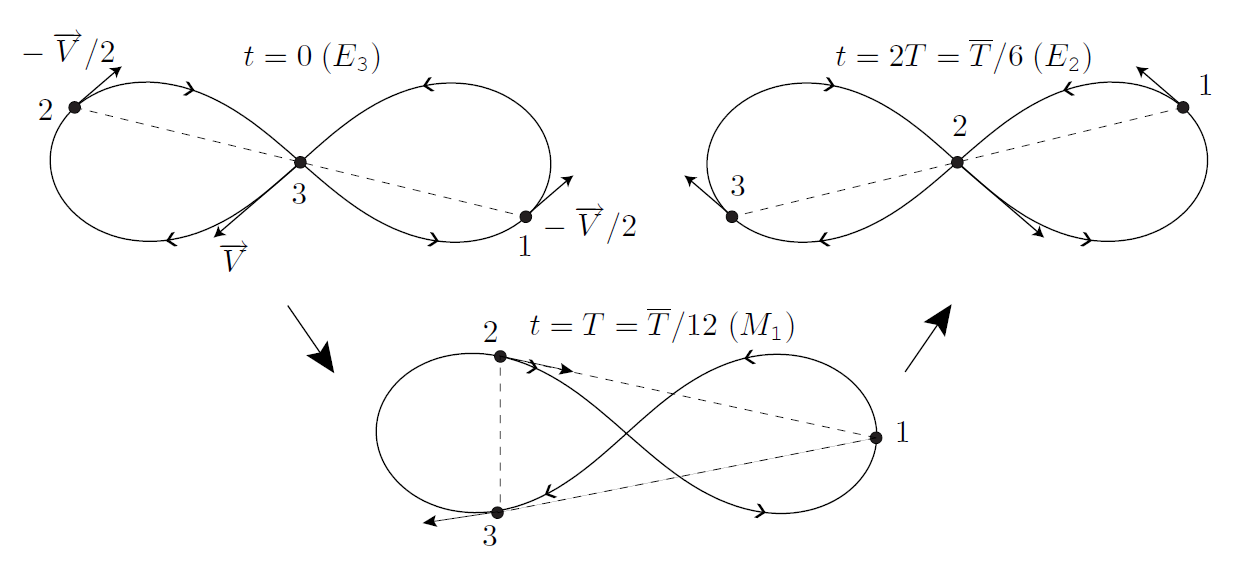
\includegraphics[width = 0.7\linewidth]{Figure_Eight_Solution.png}
	\caption{Analytically proven stable solution to three body problem. Calculated under the conditions where $G = 1$, $r_1 = -r_2 = \l( 0.970 , -0.243 \r)$, $r_3 = (0,0)$, $v_3 = -2v_1 = -2v_2 = \l(-0.932, -0.865\r)$, and $m_1 = m_2 = m_3 = 1$.}
	\label{fig:Figure_Eight_Solution}
\end{figure}
The main goal of my project is to numerically duplicate these results that have been mathematically shown to exist. 
\end{frame}


\begin{frame}

\begin{figure}
	\centering
	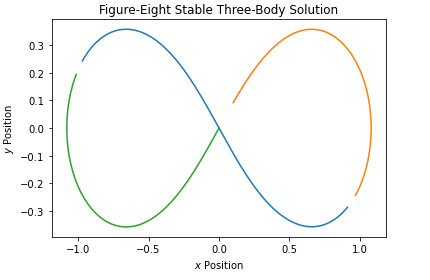
\includegraphics[width = 0.8\textwidth]{Figure_Eight_Solution_Simulation.png}
	\caption{Simulation run under the conditions where $G = 1$, $r_1 = -r_2 = \l( 0.970 , -0.243 \r)$, $r_3 = (0,0)$, $v_3 = -2v_1 = -2v_2 = \l(-0.932, -0.865\r)$, and $m_1 = m_2 = m_3 = 1$.}
	\label{fig:Figure_Eight_Solution_Simulation}
\end{figure}
\end{frame}


\begin{frame}
	\frametitle{Extensions}
	Where I want to go from here
	\begin{itemize}
		\item Investigating whether or not this orbit is stable.
		\item Use this simulation to determine the average distance of each planet from each other.
	\end{itemize}
\end{frame}

\end{document}
